\section{Introducción}
Tomando como base la metodología \textit{\acrfull{CRISP-DM}} divido el trabajo en fases, describo los procesos que se realizan en cada una de ellas y los entregables que servirán de insumo para la siguiente fase.

En las primeras fases estudio el problema y los datos. La siguiente fase, que es la preparación de los datos genero el conjunto de entrenamiento con los registros previos al año 2017, y el conjunto de validación con los registros del año 2017. En las fases de diseño y evaluación, ejecuto los algoritmos de aprendizaje no supervisado con el fin de encontrar grupos significativos con alto valor de precisión y exactitud. En la fase final se organizan los datos y  redacto el documento final.

\section{Algoritmos de aprendizaje no supervisado}
\label{par:aprendizaje_nosupervisado}
El paquete igraph\cite{igraph} de Python ofrece una variedad de algoritmos para realizar aprendizaje no supervisado. Sin embargo, por el tamaño del grafo algunos algoritmos son imposibles de usar en la práctica. Por ejemplo, el método \textit{leading edge betweenness} para detectar comunidades tiene una complejidad $O(|E||V|^2)$ en el peor caso (donde $|V|$ número de vértices y $|E|$ número de aristas). Para procesar el grafo de la red semántica de problemas se necesitaría en el peor de los casos más de 181.93 años. Los detalles de otros algoritmos para la generación de comunidades del paquete igraph se encuentran en la tabla \ref{algoritmos_igraph}.

\begin{table}[tbp]
\centering
\caption{Algoritmos de aprendizaje no supervisado del paquete igraph}
\label{algoritmos_igraph}
\begin{threeparttable}
\begin{tabularx}{\textwidth}{@{}XXXX@{}}
\toprule
Algoritmo & Observaciones & Complejidad\tnote{1}  & Cálculo de tiempo de ejecución\tnote{2} \\ \midrule
\textit{spinglass} & Comunidades basadas en la física estadística & No especificado &  \\
\textit{leading} \newline  \textit{eigenvector} & Comunidades basadas en matrices de autovectores & $O(|E|+|V|^2*steps)$, donde “steps” es atributo del algoritmo & 6.86 segundos \\
\textit{walktrap} & Comunidades basados en caminos aleatorios & $O(|E||V|^2)$ en el peor caso, $O(|V|^2 log|V|)$ en promedio, & 181.93 años en el peor caso, 38 segundos en el caso promedio \\
\textit{edge} \newline \textit{betweenness} & Comunidades basados en la métrica de centralidad intermediación & $O(|E||V|^2)$ en el peor caso & 181.93 años en el peor caso \\
\textit{fast greedy} & Comunidades basadas en optimización de la modularidad & $O(|E||V|log|V|)$ en el peor caso, $O(|E|+|V|log^2|V|)$ en promedio & 22.84 minutos en el peor caso, 0.0011 segundos en promedio \\
\textit{multilevel} & Comunidades mediante la optimización de la modularidad multinivel & En promedio lineal en grafos dispersos & 0.00064 segundos en promedio \\
\textit{label} \newline  \textit{propagation} & Comunidades basadas en la propagación de etiquetas & $O(|E|+|V|)$ & Depende del tamaño de la matriz resultante. \\
\textit{infomap} & Estructuras de comunidades que minimizan el valor esperado & No especificado &  \\ \bottomrule
\end{tabularx}
\begin{tablenotes}
    \item[1] donde $|V|$ número de vértices, $|E|$ número de aristas.
    \item[2] Cálculos basados en números de instrucciones por segundos en un procesador AMD Athlon FX-60 (Dual Core) Reloj 2.6 GHZ = 22150 MIPS.
  \end{tablenotes}
\end{threeparttable}
\end{table}

Seleccioné los siguientes algoritmos para realizar todos los experimentos de aprendizaje no supervisados, teniendo en consideración la complejidad computacional y escogiendo un representante de cada uno de los tipo de algoritmos mencionados en el capítulo anterior (divisivos, aglomerativos y optimización) (Ver sección \ref{par:algoritmos-nosupervisados}).

\subsection{Algoritmo: \textit{leading eigenvector}}\cite{Newman2006FindingMatrices.} 
\begin{itemize}
\item Complejidad: $c|V|^2 + |E|$
\item Tipo de algoritmo: Optimización
\end{itemize} 
El algoritmo \textit{Leading Eigenvector} implementado por igraph usa un algoritmo recursivo para detectar estructura de comunidades. Este algoritmo divide la red maximizando la modularidad respecto a la red original. 
 
Los métodos basados en este enfoque han tenido excelentes resultados en test estandarizados. Desafortunadamente, la optimización exhaustiva de la \textbf{modularidad} requiere grandes esfuerzos computacionales, incluyendo algoritmos voraces (\textit{greedy}), enfriamiento simulado (\textit{simulated annealing}) y optimización extrema (\textit{EO}). El algoritmo desarrollado por Newman tiene un enfoque diferente. Se reescribe la función de \textbf{modularidad} en términos de una matriz, lo cual permite expresar la tarea de optimización como un problema espectral en el álgebra lineal. Este enfoque lidera una familia de algoritmos rápidos para detectar comunidades que producen resultados que compiten con los mejores métodos previos a él.
 
\subsection{Algoritmo: \textit{multilevel}}\cite{Blondel2008FastNetworks} 
\begin{itemize}
\item Complejidad: ``lineal'' cuando  $|V|$ es aproximadamente igual a $|E|$, el algoritmo sugiere que podría ser cuadrática con los grafos completamente conectados.
\item Tipo de algoritmo: Aglomerativo
\end{itemize}
El tamaño típico de las grandes redes se cuenta en millones cuando no miles de millones de vértices. Ejemplos de estas redes son las sociales, las telefónicas móviles o la web. En esta escala se demanda nuevos métodos para recuperar información a partir de su estructura. Un enfoque prometedor consiste en la descomposición de redes en subunidades o comunidades. La identificación de estas comunidades es de crucial importancia ya que pueden ayudar a descubrir módulos funcionales desconocidos a priori, tales como tópicos en redes de información o ciber comunidades en redes sociales. Además, las meta redes resultantes, cuyos vértices son comunidades, pueden ser usadas para visualizar la estructura de la red original.
 
El algoritmo \textbf{multilevel} encuentra particiones con alta \textbf{modularidad} en grandes redes en poco tiempo y despliega una completa estructura de comunidad jerárquica para una red, dando así acceso a diferentes resoluciones de una detección de comunidades. El algoritmo se divide en dos fases que se repiten iterativamente. Asume que se empieza con una red de $N$ vértices, y cada uno de los vértices tiene un peso. Primero, se asigna una comunidad diferente a cada vértice de la red. De esta manera, en esta partición inicial hay tantas comunidades como vértices. Entonces, por cada vértice $i$ se evalúa si mejora la \textbf{modularidad} al cambiar la comunidad asociada al vértice $i$ por las comunidades en las que están cada uno de vértices adyacentes a él. El vértice $i$ es entonces puesto en la comunidad en la cual la modularidad es máxima y positiva. Si no se obtiene una ganancia positiva, entonces el vértice $i$ se mantiene en su comunidad original. Este proceso se aplica repetidamente y de manera secuencial para todos los vértices hasta que no se puede lograr ninguna mejora.
 
\subsection{Algoritmo: \textit{label propagation}}\cite{Raghavan2007NearNetworks.}
\begin{itemize}
\item Complejidad: $|V| + |E|$
\item Tipo de algoritmo: Divisivo
\end{itemize}
Cada vértice tiene una etiqueta inicial. En cada iteración del algoritmo se usa una función uniforme para determinar las aristas que son eliminadas, en el siguiente paso cada vértice adopta la etiqueta que es mayoritaria en los vértices adyacentes. A medida que las etiquetas se propagan a través de la red, grupos de nodos densamente conectados constituyen un consenso en sus etiquetas. 

Hay dos condición posibles de parada. En la primera puede ser que se llegue a la convergencia, es decir que la mayoría de los vecinos de cada vértice tengan la misma etiqueta que dicho vértice. La segunda es que se fija la cantidad máxima de iteraciones. 

Al final del algoritmo, los nodos con la misma etiqueta son conectados como comunidad. 

Las ventajas de este algoritmo sobre otros métodos es su simplicidad y su efectividad en el tiempo. El algoritmo usa la estructura de la red para guiar su progreso y no optimiza alguna métrica específica. Además, el número de comunidades y sus tamaños no se conocen a priori y se determinan cuando finaliza el algoritmo.
 
Aunque las redes con una sola comunidad satisfacen el criterio de parada, romper los enlaces aleatoriamente permite que se generen subgrafos disjuntos, evitando así que la misma etiqueta se propague por todo el grafo. En el caso de redes homogéneas que no tienen estructura de comunidades, el algoritmo identifica la red como una sola comunidad.


\section{Metodología CRISP-DM}

\begin{figure}[ht]
\caption{Metodología del trabajo de tesis}
\label{fig:Metodologia}
\centering
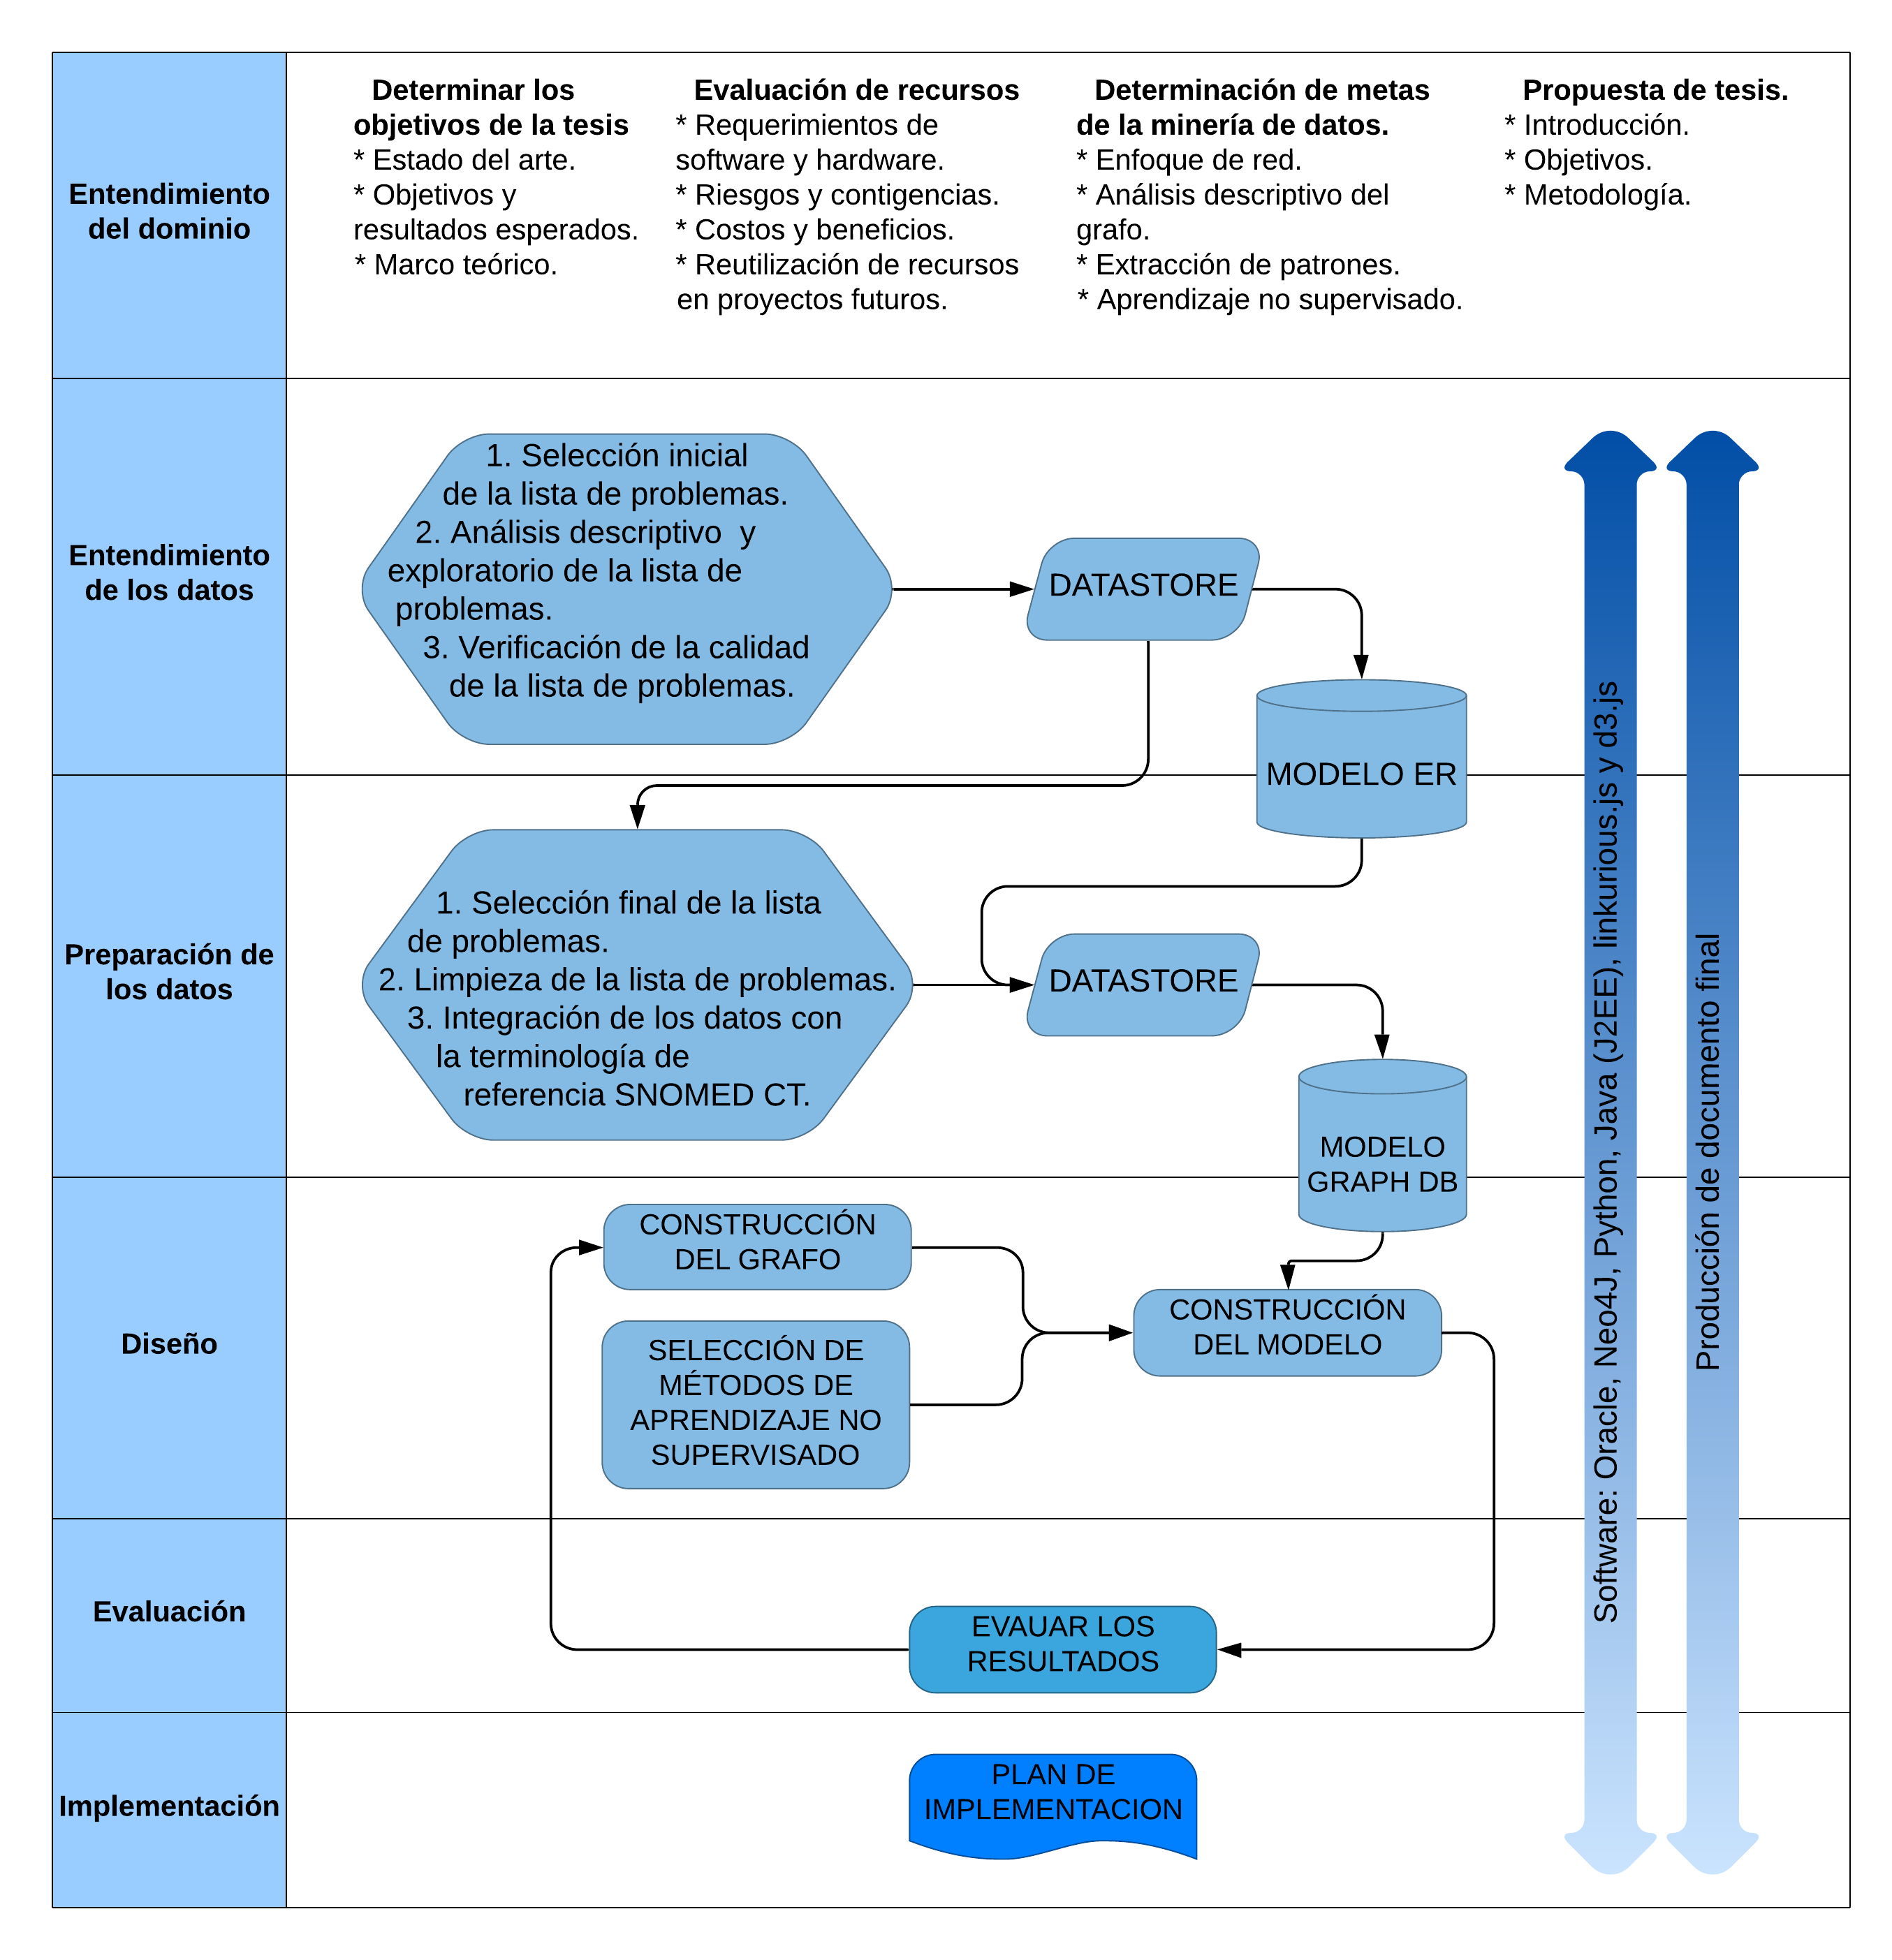
\includegraphics[width=\textwidth]{Metodologia}
\end{figure}

En el desarrollo de proyectos de minería de datos y descubrimiento de conocimiento, la metodología que más se usa es \textit{\acrshort{CRISP-DM}}. \acrshort{CRISP-DM} es una metodología independiente de dominio, por lo que puede utilizarse con cualquier herramienta de minería de datos y se puede aplicar para resolver cualquier problema de minería de datos.\cite{Marbn2009AModel}

Este trabajo se divide en seis fases (ver Figura \ref{fig:Metodologia}). Todas las fases usan transversalmente el mismo software: Oracle para el modelo de datos ER, Neo4J\footnote{Neo4j (\url{https://neo4j.com/}) es un proyecto de código abierto que permite implementar el modelo de bases de datos de grafos. Es la solución empresarial que más se usa\cite{SolidIT2019DB-EnginesDBMS}, combina la fortaleza del almacenamiento nativo de grafos y una arquitectura escalable y optimizada para asegurar un buen rendimiento en las consultas basadas en relaciones} para el modelo de datos de grafos, Python y Java para la limpieza, selección de datos y ejecución de modelos, y las librerías de javascript D3.js y linkurious.js para la visualización de los datos. 
A continuación describo lo que contempla cada fases de esta tesis.

\subsection{Fase 1: Entendimiento del Dominio.} Esta fase fue previa al trabajo de tesis en sí, y el entregable fue la propuesta de tesis. Se compone de la determinación de los objetivos, de las metas de minería de datos y la evaluación de los recursos.

Como está consignado en el primer capítulo introductorio, el objetivo es la construcción de una taxonomía de problemas, cuyas relaciones están ponderadas por su co-ocurrencia en las listas de problemas de los pacientes y sus relaciones jerárquicas con Snomed CT. Para alcanzar dicho objetivo, establecí que la meta de minería de datos es representar el conocimiento en un enfoque de red, y a partir del análisis de la red realizar la construcción jerárquica de grupos o clasificaciones de los problemas.

Para realizar esta tesis, el \acrshort{HIBA} proporcionó el acceso a los datos de la lista de problemas y la terminología Snomed CT. En términos de hardware, el \acrshort{HIBA} proporcionó el acceso a un servidor con las siguientes características:
\begin{itemize}
\item Sistema Operativo: Ubuntu 16.04.5 LTS (GNU/Linux 4.4.0-138-generic x86\_64)
\item Memoria RAM: 64 GB 
\item Espacio de almacenamiento: 760 GB
\item Número de núcleos: 8 núcleos
\end{itemize}

\subsection{Fase 2: Entendimiento de los datos.} \label{par:entendimiento_datos} Esta fase inicia con la recolección de los datos y procede con las actividades que permitan familiarizarse con ellos. El entregable se encuentra en la primera sección del capítulo 3 y contempla un análisis descriptivo para determinar la calidad de los datos de la lista de problemas, la existencia de valores atípicos (\textit{outliers})  que deben ser eliminados de los datos de entrenamiento y validación, y la construcción de contextos interesantes que permitan la formulación de hipótesis.

La construcción de  \textit{\acrshort{refset}} para agrupar problemas por contextos tiene dos metodologías: (1) determinar por extensión cuáles son los conceptos que los componen. Ya que no es fácil hacerlo por comprensión usando las relaciones subtipo de Snomed CT.  \cite{Hjen2014MethodsSets.,Lee2013AImplementations.}; o (2) El uso de \textit{\acrshort{refset}} públicos para comparar el cubrimiento  con los \textit{\acrshort{refset}} generados aquí \cite{Lee2013AImplementations.}. Esta tesis usa la segunda metodología. Se usa aprendizaje no supervisado para generar grupos con los registros en la lista de problemas y los contextos en los cuales se realizaron los registros.  Si hay solapamiento de conceptos entre los contextos, se fusionan los contextos. Finalmente si hay \textit{\acrshort{refset}} similares en Kaiser Permanente \acrshort{CMT} entonces se evalúa el cubrimiento con ellos (Ver sección \ref{par:cubrimiento}).  Posteriormente las decisiones finales sobre fusión de  contextos son evaluados manualmente por la residencia de informática médica.  

Los contextos nivel asistencial y grupo etário tienen una cardinalidad pequeña, 8 y 9 respectivamente. Por el contrario, las áreas jerárquicas tienen una cardinalidad grande, inicialmente son 601 áreas jerárquicas. Las áreas jerárquicas tienen un proceso extra para evaluar sus solapamientos y así agruparlas dentro de las más significativas. Este último proceso se realiza con el algoritmo de aprendizaje supervisado StanfordNLP ColumnClassifier \cite{manning-EtAl:2014:P14-5}. La variable objetivo del algoritmo de clasificación es  el servicio al que pertenecen los conceptos, un algoritmo de clasificación tendría mayor dificultad para predecir el servicio si hay muchos conceptos similares entre ellos, por lo tanto serían candidatos a fusión. La dificultad se mide con valores de \textit{F1 score}\footnote{\textit{F1-Score} es un valor único que pondera la precisión y la exhaustividad. \textit{F1 score} hace referencia a la efectividad de un modelo y es conocida en la estadística como una proporción de acuerdo específico ya que se aplica a una clase específica, la clase positiva.\cite{Powers2011Evaluation:Correlation}} bajos. La residencia de informática médica determina manualmente si concuerda con la fusión de los contextos.


\subsection{Fase 3: Preparación de los datos.} Esta fase se compone de la extracción de los datos desde el modelo ER, limpieza y transformación de los datos con los que se realizan los modelos. El entregable es el conjunto de datos de entrenamiento y validación. El conjunto de entrenamiento contiene los registros de problemas previos al 2017. El conjunto de validación contiene los registros que ingresaron a la \acrshort{HCE} en el 2017 y cuyos pacientes tengan una lista de problemas no vacía.

\subsection{Fase 4 y 5: Diseño y evaluación.} \label{par:disenho_evaluacion} Esta fase se compone de las siguientes tareas:
\begin{itemize}
\item Construcción del grafo: Determinación del modelo de datos y carga de la base de datos de grafos Neo4j. Usando los datos de entrenamiento se obtiene un grafo cuyos vértices son los problemas y las aristas son las co-ocurrencias en los pacientes (Red de Problemas) y las relaciones dadas por la terminología de referencia Snomed CT (Red semántica de problemas). Los vértices son etiquetados con información contextual: ámbito o nivel de asistencia, grupo etario y área jerárquica.  

\item Caracterización de las redes y búsqueda de patrones en las redes:
\begin{itemize}
\item Determinar si la distribución de la red es libre de escala: La hipótesis nula es que los grados de los vértices se distribuyen según la ley de potencias. Se estima la función de distribución acumulativa \acrshort{cdf}, en el caso de que el p-valor de la función no permita rechazar la hipótesis nula entonces se compara el estadístico \textit{log-likelihood ratio} con otras distribuciones.
\item Análisis de estructuras de comunidad: Métricas para comparar cuantitativamente los grafos de la red de problemas y la red semántica de problemas. Se evalúa si los grafos presenta evidencias de tener comunidades: coeficientes de agrupamiento, longitud media del camino mínimo entre nodos y promedio de grados. El cálculo de estas métricas están disponibles en los paquetes igraph\cite{igraph} y networkx\cite{SciPyProceedings_11} de python.
\end{itemize}

\item Aprendizaje no supervisado: Aplicación de algoritmos de aprendizaje no supervisado a la red de problemas y la red semántica de problemas. Por las limitaciones en hardware no se puede procesar el grafo completo de la red semántica de problemas, se realizan las siguientes tareas con sub-grafos de problemas que co-ocurran en \num{10000}, \num{1000}, \num{100}, \num{10} y \num{5} pacientes:
\begin{itemize}
    \item Identificación de grupos o \textit{clusters} significativos que comparten patrones comunes de atributos y relaciones. 
    \item Cada uno de los vértices que contiene el \textit{cluster} tiene calculada las medidas de centralidad para entender su influencia dentro de la red. 
    \item A los grupos encontrados se les realiza un test para evaluar la significancia de los \textit{clusters}, los siguientes pasos son realizados 1000 veces:
    \begin{itemize}
\item  se generan aleatoriamente aristas en el grafo
\item  se aplican los algoritmos de aprendizaje no supervisado
\item  se evalúa si la modularidad es superior a la modularidad del grafo original.
\end{itemize}
\end{itemize}

\item Validación de los resultados: 
\label{par:evaluacion-resultados}
Teniendo en cuenta las directrices de recuperación de información \cite{Manning2008,Hersh1994OHSUMED:Research}, el conjunto de validación tiene tres componentes: 

\begin{itemize}
\item \textbf{El conjunto de pruebas}: se conforma de los problemas registrados previamente y los valores del contexto (nivel asistencia, grupo etario y área jerárquica), que representan la consulta, y el problema a predecir que representa la respuesta correcta
\item \textbf{Los conceptos de Snomed CT a ser recuperados}: la lista previa de problemas permite identificar los subgrafos, y los valores de contexto permiten filtrar los vértices. De esta manera, creo una \textbf{lista de sugerencias} por cada uno de los registros del conjunto de pruebas.
\item una medida de relevancia por cada par de consulta-concepto recuperado, esta medida es la \textbf{transitividad} o la \textbf{distancia semántica}, y permite un ordenamiento de los resultados. Estas medidas están definidas en el capítulo introductorio (Ver sección \ref{par:efecto-comunidades}).
\end{itemize}

Lo que se evalúa es si los vértices que pertenecen al mismo \textit{cluster} permiten completar los problemas faltantes en la lista de los problemas de los pacientes del conjunto de datos de validación. Esta evaluación se realiza con la lista de problemas previas al 2017 y los contextos para seleccionar y filtrar la  \textbf{lista de sugerencias}, y predecir los problemas registrados en el 2017.

Se evalúan por separado la capacidad predictiva (precisión y exactitud) de los grupos encontrados a partir del grafo de la red de problemas y del grafo de la red semántica de problemas. También son evaluadas las capacidades predictivas filtrando el contexto: ámbito o nivel de asistencia, grupo etario y área jerárquica, sólo en red de problemas. La precisión y la exactitud (\textit{accuracy}) se definen como:

\begin{equation}
Exactitud = \frac{\text{Verdaderos positivos}+\text{Verdaderos negativos}}{\text{Total de los datos}}
\end{equation}

\begin{equation}
Precision = \frac{\text{Verdaderos positivos}}{\text{Verdaderos positivos}+\text{Falsos positivos}}
\end{equation}

La exactitud suma los verdaderos positivos, que son los casos en los que la lista de sugerencia contiene la respuesta correcta, y los verdaderos negativos, que son los casos en los que la lista de sugerencias esta vacía y el problema a predecir no está dentro de los conceptos de Snomed CT a ser recuperados, y los divide en la totalidad de los datos de prueba. Se evalúa también una versión más flexible de verdadero positivo, donde se define una distancia tolerable de longitud media del camino mínimo entre la respuesta correcta y alguno de los conceptos de la lista de sugerencias. Esta distancia se estableció de tamaño 3, e indica similitudes entre un concepto y los descendientes que están hasta dos vértices de distancia, o conceptos descendientes del mismo padre, como se ilustra en la figura \ref{fig:distancias_semanticas}.

\begin{figure}[ht]
\caption{Modelo de datos}
\label{fig:distancias_semanticas}
\centering
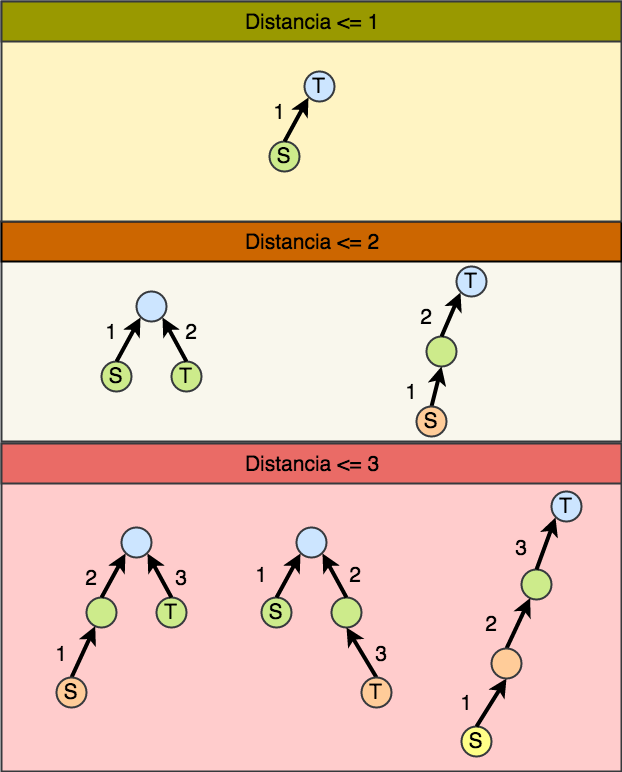
\includegraphics[width=0.5\textwidth]{distancias_semanticas}
\end{figure}
 
La precisión evalúa cuántas veces la lista de sugerencias no vacía tiene la respuesta correcta, dividido las veces que se obtuvo una respuesta positiva. Teniendo en cuenta que las listas de sugerencias son de un tamaño $n$ ordenados según la relevancia, las medidas son llamadas precisión al $n$ o $P@n$ y exactitud al $n$ o $Acc@n$.

 \end{itemize}
 
\subsection{Fase 6: Implementación.} En la última fase organizo los datos y redacto el documento final de la tesis. El plan de implementación en la organización de los datos y los servicios de terminología del \acrshort{HIBA} no hacen parte de los entregables de esta tesis.




